\documentclass[a4paper]{jpconf}
\usepackage[utf8]{inputenc}

\usepackage{graphicx} % Required for including pictures
\usepackage{listings}
\usepackage{float} % Allows putting an [H] in \begin{figure} to specify the exact location of the figure
\usepackage{wrapfig} % Allows in-line images such as the example fish picture
\usepackage{color}


\begin{document}


\lstset{frame=tb,
  language=perl,
  aboveskip=3mm,
  belowskip=3mm,
  showstringspaces=false,
  columns=flexible,
  basicstyle={\small\ttfamily},
  numbers=none,
  breaklines=true,
  breakatwhitespace=true,
  breaklines=true,
  frame=none
}


% Title Page
\title{
DPM Evolution: a Disk Operations Management Engine for DPM}

\author{Andrea Manzi, Fabrizio Furano, Oliver Keeble, Georgios Bitzes}

\address{CERN IT}

\ead{amanzi@cern.ch, furano@cern.ch, okeeble@cern.ch, georgios.bitzes@cern.ch}

\begin{abstract}

The DPM (Disk Pool Manager) project is the most widely deployed solution for storage of
large data repositories on Grid sites, and is completing the most important upgrade
in its history, with the aim of bringing important new features, performance
and easier long term maintainability.
Work has been done to make the so-called "legacy stack" optional, and substitute
it with an advanced implementation that is based on the fastCGI and RESTful technologies.
Beside the obvious gain in making optional several legacy components that
are difficult to maintain, this step brings important features together with
performance enhancements. Among the most important features we can cite the
simplification of the configuration, the possibility of working in a totally
SRM-free mode, the implementation of quotas, free/used space on directories,
and the implementation of volatile pools that can pull files from external
sources, which can be used to deploy data caches.
Moreover, the communication with the new core, called DOME
(Disk Operations Management Engine) now happens through secure HTTPS channels
through an extensively documented, industry-compliant protocol.
For this leap, referred to with the codename "DPM Evolution", the help of the
DPM collaboration has been very important in the beta testing phases,
and here we report about the technical choices and the first site experiences.

\end{abstract}



\newpage % Begins the essay on a new page instead of on the same page as the table of contents


%----------------------------------------------------------------------------------------
%	TABLE OF CONTENTS
%----------------------------------------------------------------------------------------


\section{Dome}

DOME (Disk operations Management Engine) is a robust, high performance server that manages the operations of a DPM cluster. DOME is built on the FastCGI technology,
and uses HTTP and JSON to communicate with clients.
This initiative aims at augmenting the Disk Pool Manager (DPM) system so that its core coordination functions and inter-cluster communication paths are
implemented through open components, and following contemporary development approaches headed to performance, scalability and maintainability. Among our goals we cite:

\begin{itemize}
 \item Making optional all the so-called legacy components that are provided by the \textit{lcg-dm} code tree, namely \textit{libshift}, \textit{rfiod},
 \textit{dpm(daemon)}, \textit{dpnsdaemon}, \textit{CSec} and others.
 \item provide a software infrastructure where adding new coordination features is easier than with \textit{lcg-dm}
 \item provide full support for asynchronous calculation of file checksums of multiple types
 \item provide support for checking the consistence of replicas through their checksums
 \item provide structure, hooks and callouts that allow the usage of DPM as a fast and large \textit{file cache}
 \item having a unified configuration file that is readable and synthetic, as opposed to the \textit{lcg-dm} approach of having several configuration
 files here and there, all with differently over-simplified syntax rules (or no syntax at all, e.g. \textit{/etc/NSCONFIG})
\end{itemize}

The DOME component has the shape of a \textit{fastCGI} daemon, and has to be triggered by the Apache instances running in the DPM head node and
in all the DPM disk servers. A configuration option defines whether it is running as head node or disk server.

For simplicity of expression, in this document we may refer to these modalities as two different components, named \textit{DOMEhead} and \textit{DOMEdisk}.
In practice, these refer to the same component which has been given a different command-line flag to enable/disable a different command set,
implemented in the same software skeleton.\\

DOME is primarily a service provider for the \textit{dmlite} framework, through the dmlite plugin called DOMEAdapter.\\

\section{DOME: Main features}
DOME has two modalities: headnode and disknode, which respectively represent evolutions of the \textit{dpm} daemon and of \textit{rfiod}, together with \textit{libshift} and \textit{Csec}.
The functionalities are roughly as follows:
\begin{itemize}
 \item headnode: general coordination function
 \subitem spreads load (PUT, GET, checksums) towards the available disk nodes
 \subitem keeps an in memory status of the DPM disk/pool topology with disk sizes and free space
 \subitem keeps an in memory status of the ongoing asynchronous checksum calculations
 \subitem keeps an in memory status of the ongoing asynchronous file callouts
 \subitem queues and dispatches to disk nodes the requests for asynchronous checksum calculations that have to be delayed for load balancing reasons
 \subitem queues and dispatches to disk nodes the requests for asynchronous file callouts that have to be delayed for load balancing reasons

 \item disknode: local disk and space-related services
 \subitem Allows to \textit{stat} individual physical files and directories
 \subitem Allows to \textit{statfs} filesystems to get used and free space
 \subitem Allows the local submission of checksum calculations
 \subitem Allows the local submission of file callouts
\end{itemize}

The historical tunnelling feature provided by the \textit{rfio} infrastructure (and used by gridftp in some boundary scenarios)
is implemented by DOMEAdapter directly on the top of HTTP, hence namely it does not use the DOME server.\\


The main difference from the legacy components is that DOME does not apply authorization again for individual user file
access, as this task is already accomplished by the dmlite frontends. DOME only checks that the sender of a request is authorized to
send requests, in a way that is similar to the libshift "root mode". DOME applies strong, industry standard authentication protocols to this task.\\
Authentication in DOME is zero-config for the regular cases (one head node and multiple disk servers), and flexible enough
to add arbitrary identities that will be allowed to send commands to it.\\

\textbf{DOME is protocol-agnostic. Its concepts of logical file name and physical file name are not linked to a particular data/metadata transfer protocol.
DOME manages paths and filenames, not URLs. URLs can be constructed by the DPM frontends starting from the pfn or lfn information given by DOME.}


\subsection{From spacetokens to quota tokens}
Historically, DPM does space accounting through a set of individual named space reservations, kept in the DB in the head node, and associated to pools.\\
Semantically, space reservations are named reservations of a part of the space of a disk pool. Requests to write a replica specify a pool
that has to host the replica, hence ultimately the replica will be subject to the space reservations.\\

One of the weakest points in this schema is that the writer has to know technical details of the destination storage, to be able to write
and be properly accounted for.\\

Another historical weak point is that calculating good numbers for the space occupancies can be a challenging exercise, especially if the structure of the pools
has been modified in the years.\\
The development direction of DOME is to evolve this mechanism towards \textit{subdirectory\-based space accounting}, instead than pool-based.\\

In subdirectory-based space accounting, every subdirectory at less than N levels from the root is kept updated with the total size of the replicas
of files that reside in that directory subtree.\\

This \textit{subdirectory size} together with the information on free/used space in the pools associated to these subdirectory tree
can then be used to compute the needed space occupancy numbers.

DOME uses the records describing spacetokens that are kept in the head node DB, with minimal modification. Their meaning is slightly changed,
into semantically representing a quota on one and only one directory subtree. From this point on, we will refer to them as \textit{quotatokens},
whose behavior is similar to that of an old spacetoken associated to a directory.\\

A \textit{quotatoken} attached to a directory subtree \textbf{overrides others that may be attached to its parents}.\\
If a directory content (counting all the replicas) exceeds the quota spacified by the quotatoken that influences it,
then new PUT requests on that dir will be denied.\\

As a summary, the meaning of a quotatoken specifying a quota of N on poolX, associated to directory "/dir1" is \textit{give poolX as
space for hosting the files that will be written into \/dir1. Do not allow more than N terabytes to be hosted there}.\\

\subsection{Pools and filesystems}
A pool is a logical group of mount points in individual disk servers that are used to store replicas.\\

DOME uses the same concept of Pool than the historical DPM, hence the "Pool management" functionalities
of the legacy lcg-dm components continue to work mostly as they were.\\

A Pool can be associated to a directory subtree by creating suitable quotatokens that describe the individual associations.\\

A Pool assigned to a subtree acts as a sort of "replication domain". Replicas of files belonging to that subtree
are stored in filesystems belonging to this pool. Multiple replicas are spread through different file systems.\\

We would like to emphasize that only one pool can be assigned to the same directory subtree (e.g. /dpm/cern/ch/home/dteam/scratch).
Writes into this subtree will be space-balanced between all the filesystems composing the pool assigned to it. A pool instead can be associated
to any number of quotatokens (and hence, directories).\\

\subsection{Open checksumming}
DOME supports requests for checksums of arbitrary kind. It can:\\

\begin{itemize}
 \item return the corresponding checksum that is stored in the name space
 \item choose an appropriate replica of the file and tell to the disk node managing it to calculate its checksum
 \item force the recalculation of the checksum and store it into the name space
\end{itemize}

The checksum calculation request may be queued in the head node, in memory. The architecture is designed to be self-healing in the case the checksum
calculations do not end correctly, or some machines are restarted.





\section{Tech}

The architecture of DOME is expandable, through the usage of an open, human-readable protocol (JSON) and through proper design.\\


\subsection{Architecture}
Figure \ref{figdomedisk} shows the main components of DOME that are in action in a disk server.\\
Requests come through Apache already authenticated and referring to the two possible paths that
refer either to the filesystems or to the dome command path which starts with \lstinline{/domedisk}.
Another detail that characterizes a disk server for DOME is the ability to execute tasks like checksum calculations
and file pulls from external sources. These tasks, following a logic that is based on time, report their status
to the head node, which uses this information to keep its queues updated.\\
 
\begin{figure}
\begin{center}
 \includegraphics[width=10cm,keepaspectratio=true,angle=-90,origin=c]{./pics/domepics_disk.eps}
 % domepics_disk.ps: 0x0 pixel, 300dpi, 0.00x0.00 cm, bb=
 \caption{Simplified diagram of DOME in a disk node}
 \label{figdomedisk}
\end{center}
\end{figure}

A DOME head node is slightly more complex than a disk server, and its internal structure is
visible in Figure \ref{figdomehead}.\\
Requests come through Apache already authenticated and referring to the two possible paths that
refer either to the logical name space ( \lstinline{/dpm} ) or to the dome command path which starts with \lstinline{/domehead}.
A head node can contact external systems to get information about remote files, and queues in memory the requests for checksum calculations and remote file pulling.\\


\begin{figure}
\begin{center}
 \includegraphics[width=10cm,keepaspectratio=true,angle=-90,origin=c]{./pics/domepics_head.eps}
 % domepics_disk.ps: 0x0 pixel, 300dpi, 0.00x0.00 cm, bb=
 \caption{Simplified diagram of DOME in a head node}
 \label{figdomehead}
\end{center}

\end{figure}

\subsection{Security}
DOME by default accepts requests from the disk servers of the cluster it manages. This mechanism is based on secure HTTPS handshakes.\\
Additionally, the configuration file can specify criteria to accept requests that come to DOME. These criteria have the form
of a list of allowed DNs (taken from X509 certificates).\\

The typical configuration uses HTTPS in the frontend configuration, to enforce the usage of a valid certificate.\\

\subsection{Checksum queuer}
 DOME internally queues and schedules checksum calculation requests in the head node.\\
 No more than N checksums will be run per disk mount\\
 No more than L checksums will be run per disk server\\
 No more than M checksums will be run in total\\

 Checksum requests are queued in memory and dispatched to suitable disk nodes that become available with respect to the mentioned criteria. The disk nodes instances constantly update the head node about the running checksums, hance there is no need for persistence,
 and the system will self-heal on restarts of the head node. When finished calculating a checksum, a disk node will notify the head node and pass the result (or failure).\\
 Eventually in the future memcached can be used for queue synchronization purposes. This evenience would require more development effort, and would have the
 advantage of making the DOME service able to scale horizontally.\\

\subsection{File pulls queuer}
DOME internally on the head node queues and schedules requests for file pulls from external locations
 No more than N pulls will be run per disk mount\\
 No more than L pulls will be run per disk server\\
 No more than M pulls will be run in total\\

The pull itself is implemented as a simple callout in the disk server, that can invoke any file movement mechanism, from
\textit{dd} to create an empty file to a simple copy to ultracomplex multi hop FTS xfers.
The pull callout in the disk server is complemented by a stat callout, which is able to stat an external system for the presence of an offline file.\\
This mechanism should be polished enough to support the construction of simple file caches,
without necessarily needing external, complex components. Invoking FTS instead than \textit{dd} or \textit{davix-get} must be an option.\\


Pull requests are queued in memory and dispatched to disk nodes that match the request and become available. Please note that stat requests to external systems are not queued.\\
The disk nodes instances constantly update the head node on the running callouts, hance there is no need for persistence,
and the system will self-heal on restarts of the head node. When finished pulling a file, a disk node will notify the head node and pass the result (or failure).\\

Eventually memcached can be used for queue synchronization purposes, only if it turns out that even in SOME cases the code is not totally
preventing the spawning of new processes (which has never to happen!!!). This evenience would require more development effort, and would have the
advantage of making the dpm service able to scale horizontally.\\

\subsection{Only one process}
 The fastcgi app named DOME consists in one process which manages multiple internal thread pools.\\

 


\section{Application programming interface}

Historically DPM implements low level functionality that is used by frontends to coordinate
their activities of exposing data access protocols to clients.\\
In some cases, the historical DPM API has been also exposed to clients/users, eventually through a
Storage Resource Manager (SRM) server.

DOME is not supposed to be used by remote clients and users. Users interact with DPM through a suitable frontend (e.g. gridFTP, xrootd, Apache) that
relies on the services of dmlite and DOME in the background.




\section*{References}
\begin{thebibliography}{9}
\bibitem{iopartnum} IOP Publishing is to grateful Mark A Caprio, Center for Theoretical Physics, Yale University, for permission to include the {\tt iopart-num} \BibTeX package (version 2.0, December 21, 2006) with  this documentation. Updates and new releases of {\tt iopart-num} can be found on \verb"www.ctan.org" (CTAN). 
\end{thebibliography}

\end{document}
